\documentclass[t]{beamer}

\usepackage[utf8]{inputenc}


\title{Project Progress}
\subtitle{What constitutes ``Home field advantage" in the NFL?}
\author{Chau Nguyen}
\date{\today}



\begin{document}

\frame{\titlepage}

\begin{frame}
\frametitle{Background \& Motivation}
 {I want to study ``home field advantage" in the National Football League (NFL). When football analysts and pundits discuss ``home field advantage", it usually is a combination of a few things:}
\pause
\begin{itemize}
	\item<2->{Distance traveled: The Home team does not have to travel to play the game (there are rare exceptions). This helps with their ability to rest, practice, and game plan.}
	\item<3->{The Away team is at an even more disadvantage if they had to travel across timezones for the match up.}
	\item<4->{With fans in the stand, the Home crowd is usually silent during the Home team's Offensive snaps (so that the Quarterback can ``read" the opposing Defense and make adjustments to the play before the snap).}
	\item<5->{On the other hand, during the Away team's Offensive snaps, the Home crowd is encouraged to get loud - therefore the opposing QB can't do the same.}
\end{itemize}
\end{frame}
%%%%%%%%%%%%%%
\begin{frame}
\frametitle{Background \& Motivation}
The situation is different in 2020. Many stadiums are required to limit fan attendance to a very low number to mitigate covid risks. Players have commented on how eerily quiet and different the game day atmosphere has been this year. 


With that in mind, I wanted to see if I could build a model that quantifies ``Home field advantage" in a normal year. 
\begin{itemize}
\item<1->{Do Home teams really win more?}
\item<2->{What is it about the Home Stadium that helps a team win?}
\item<3->{Is it the Stadium itself? The Home fans in attendance?}
\item<4->{Or is it the lack of travel that helps?}
\end{itemize}

{If the model does well between the training and test datasets, I want to use it on game outcomes for the 2020 Season and see what comes from there.}


\end{frame}

\begin{frame}
\frametitle{Overview of the NFL}
	
	\begin{itemize}
	\item{Currently, there are 32 teams in the NFL, divided into 2 conferences: the National Football Conference (NFC) and the American Football Conference (AFC). Each conference is divided into 4 divisions: North, South, East, West - each with 4 teams. }
	
	
	\item<2-> This has not always been the case before the ``realignment" in 2002, the landscape of the NFL looked quite different. 	
	

\end{itemize}
\end{frame}

\begin{frame}
\frametitle{Overview of the NFL}
\centering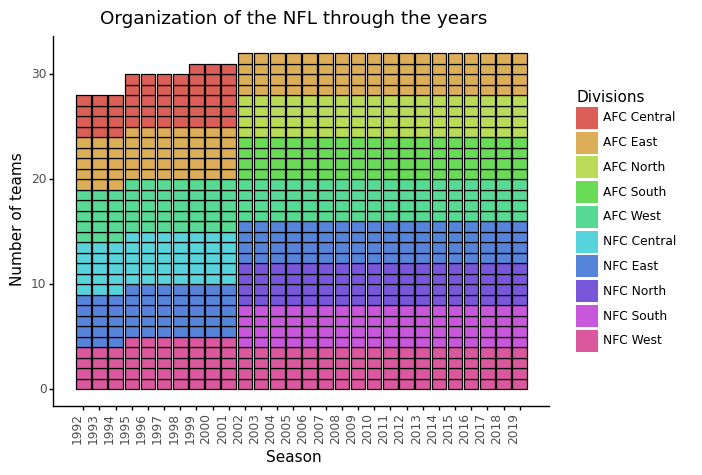
\includegraphics[width=\linewidth]{../09_figures/plot_div_team_count.png}
\end{frame}

%%%%%%%%%%%%%
%%%%%%%%%%%%%%%%%%%%% 

\begin{frame}
\frametitle{Methods and approaches I considered using}
\begin{itemize}
\item<1-> Pro-Football-Reference.com has attendance data for every NFL game starting in 1992 - this was my starting point.
\item<2-> I wanted to practice webscraping and data wrangling with Python, so I set out to write scrapers for the data I needed - mostly from Wikipedia and Pro-Football-Reference.
\item<3-> I would calculate the ``distance traveled" for each team using the distance measured between their Home stadium and the stadium they're playing at.
\item<4-> I can also calculate the amount of time each team has had to rest inbetween games. 
\item<5-> I want to format my dataset into a dyadic panel and use Machine Learning to study the difference between each pair.

\end{itemize}
\end{frame}


%%%%%%%%%%%%%%%%%%%%%%%%%%%
\begin{frame}
\frametitle{Methods and tools used to date, and rationale for their use}
\begin{itemize}
	\item<1->{I have written many scrapers for Wikipedia using BeautifulSoup, because a lot of the time the read\_html function in pandas does not give me what I need.}
	\item<2->{Even then, because of the data challenges above, I still needed to go in and clean up the scraped data manually - this was the most time consuming part.}
	\item<3->{Why?}
\end{itemize}
\end{frame}




%%%%%%%%%%
\begin{frame}
\frametitle{Challenge 1: Team Names, Stadiums and Game Locations}
\begin{itemize}
\item<1-> NFL franchises move cities and rename themselves over the years.
	\begin{itemize}
	\item<2->{Cleveland Rams (1936 - 1945, LA Rams (1946-1994), St. Louis Rams (1995 - 2015), LA Rams (2016 - present).}
	\item<2->{The team previously known as "Washington Redskins" is being called "Washington Football Team" temporarily beginning 2020 until the franchise finds a new name.}
	\end{itemize}
\item<3-> Unique games such as the NFL International Series played in London and Mexico City every year, or the Bill Toronto Series.
\item<4-> Games being moved because of "Act of God" events
	\begin{itemize}
		\item<5->{The New Orleans Saints played their 2005 season on the road due to Hurricane Katrina - their "Home" games were played in nearby stadiums, but not the Superdome.}
	\end{itemize}
		
		\end{itemize}

\end{frame}

\begin{frame}
\frametitle{Challenge 1: Team Names, Stadiums and Game Locations}
\pause
\centering\includegraphics[width=\linewidth]<2->{../09_figures/plot_city.png}

\end{frame}

%%%%%%%%%%%%%%%%%%%%%%%%%%%%%
\begin{frame}
\frametitle{Challenge 2: Even in the same stadium, maximum capacity is not static}

\pause

\centering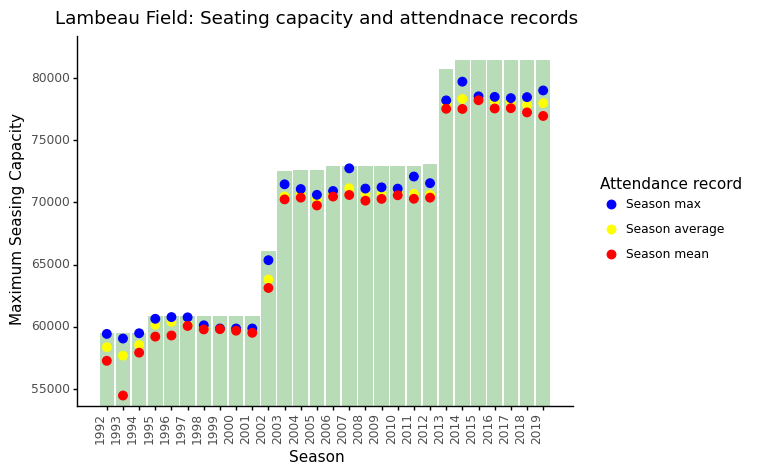
\includegraphics[width=\linewidth]{../09_figures/plot_lambeau.png}

\end{frame}






%%%%%%%%%%%%%



\begin{frame}
\frametitle{Preliminary results and conclusions}

\begin{itemize}
\item<1->{I do not have any preliminary results yet, because I'm still not 100\% happy with my data (as I'm making this presentation, I saw a few things that needed improving).}
	\begin{itemize}
	\item<2->{For example, take a look at this graph}
	
\centering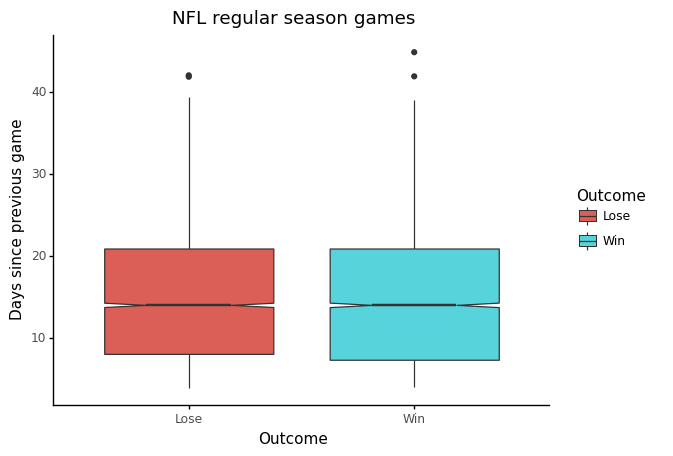
\includegraphics[width=\linewidth]{../09_figures/plot_timerest_wrong.png}
	\end{itemize}
\end{itemize}
\end{frame}

\begin{frame}
\frametitle{Where I am right now}

\begin{itemize}
\item<1->{I do not have preliminary results yet, because I'm still not 100\% happy with my data (as I'm making this presentation, I saw a few things that needed improving).}
	\begin{itemize}
	\item<2->{If you are not familiar with the NFL - teams play each other every weekend. Then why is the average number of days between the losing team and the winning team around 14 days?}
	\item<3->{This has to do with how I cleaned my data before turning it into a dyad. I will have to revisit this and fix it.}

	\end{itemize}
\end{itemize}
\end{frame}	

\begin{frame}
\frametitle{Where I am right now}
\begin{itemize}
\item<1->{I have data for 7,292 games across 28 NFL seasons from 1992 to 2019.}
\item<2->{This is a snippet of my (dyad) data at the moment (ignore the incorrect Time\_rest\_days).}

\centering\includegraphics[width=\linewidth]<2->{./data_snippet.png}
\item<3->{I am not entirely confident in studying dyadic data.}
\end{itemize}
\end{frame}

%%%%%%%%%
\begin{frame}
\frametitle{Lessons learned so far}

\begin{itemize}
\item<1->{Webscraping is not easy, even from a prety standardized site like Wikipedia.}
\item<2->{I learned a lot about parsing HTML data (which was one of my original goals when I started this project).}
	\item<3->{Instead of Markdown, I am using pure {\LaTeX}  to make this presentation.}

\end{itemize}
\end{frame}
%%%%%%%%%%%%%%%%%%
\begin{frame}
\frametitle{Mitigation plans}
\begin{itemize}
\item<1->{I still need to do more cleaning to my dataset - but I think I'm almost there.}
\item<2->{I do not think I will have enough time to scrape weather/ dome/ stadium size data as Professor Dunford suggested in my project proposal.}
\item<3->{My priorities right now are to finish up the very last bits of cleaning fixes to the data, and move onto the machine learning part.}
\item<4->{I think it's realistic to think that I will not be able to complete the 2020 season part of this project - but if things go well I do want to keep playing with the models even after the semester ends.}



\end{itemize}
\end{frame}

%%%
\begin{frame}
\frametitle{Thank you!}%%     1
Thank you for taking your time to listen to my presentation. Any feedback is greatly appreciated!
\end{frame}
\end{document}
